\section{Mise en œuvre matérielle et synthèse sous Vivado}

Pour rendre le système synthétisable sur un FPGA AMD (anciennement Xilinx) sous Vivado, certaines modifications et précautions sont nécessaires. Le code matériel doit être parfaitement compatible avec les contraintes de synthèse et les ressources logiques disponibles sur le composant cible.

\subsection{Modification du code existant}

Dans notre projet, le processeur (RISC-V) est écrit en Verilog tandis que la mémoire et le niveau supérieur (\textit{Top-Level}) sont en VHDL. Pour garantir la synthétisabilité de l'ensemble mixte :
\begin{itemize}
    \item Un nettoyage des constructions de simulation non synthétisables a été réalisé (comme la suppression ou l'isolation des instructions de debug de type \texttt{\$display} dans le processeur Verilog).
    \item Les sensibilités d'horloge et de réinitialisation ont été standardisées pour correspondre aux attentes des outils de synthèse FPGA.
\end{itemize}

\subsection{Contraintes de synthèse et préservation des signaux sous Vivado}

Durant l'étape de synthèse, l'outil analyse le design et applique des optimisations agressives (suppression de la logique jugée redondante ou non connectée aux broches physiques de sortie). Étant donné que notre système fonctionne de manière autonome en interne sans relier tous les signaux mémoire à des broches externes du FPGA, Vivado pourrait être tenté d'optimiser et de supprimer les bus d'interconnexion.

Pour empêcher cette suppression indésirable et conserver une visibilité complète sur la netlist, nous avons appliqué l'attribut de synthèse \textbf{\texttt{DONT\_TOUCH}} sur les signaux intermédiaires du top-level (Listing \ref{lst:top_level_modifie}).

\begin{lstlisting}[language=VHDL, caption={Extrait du Top-Level système avec application de l'attribut DONT\_TOUCH sous Vivado}, label={lst:top_level_modifie}]
attribute DONT_TOUCH : string;
attribute DONT_TOUCH of mem_addr      : signal is "true";
attribute DONT_TOUCH of mem_wdata     : signal is "true";
attribute DONT_TOUCH of mem_rdata     : signal is "true";
attribute DONT_TOUCH of mem_we        : signal is "true";
attribute DONT_TOUCH of quadram_addr  : signal is "true";
attribute DONT_TOUCH of quadram_wdata : signal is "true";
attribute DONT_TOUCH of quadram_rdata : signal is "true";
\end{lstlisting}

\subsection{Analyse de la synthèse et de l'implémentation}

Ci-dessous, les différentes vues issues de l'outil Vivado illustrant les étapes de synthèse et d'implémentation :

\begin{figure}[H]
    \centering
    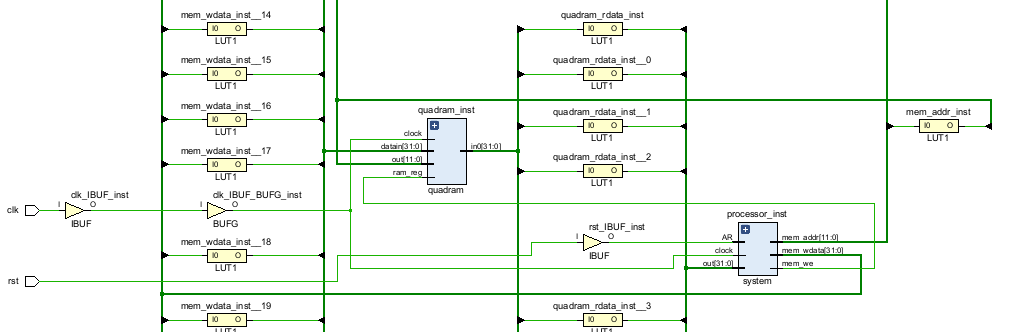
\includegraphics[width=0.99\textwidth]{Images/6_Sche_synth_1.png}
    \caption{Schéma global de synthèse}
    \label{fig:sche_synth}
\end{figure}

Dans cette première capture, nous observons le schéma global de synthèse du design, où les blocs principaux (processeur et QuadRAM) sont interconnectés.

\begin{figure}[htbp]
    \centering
    \begin{subfigure}[b]{0.48\textwidth}
        \centering
        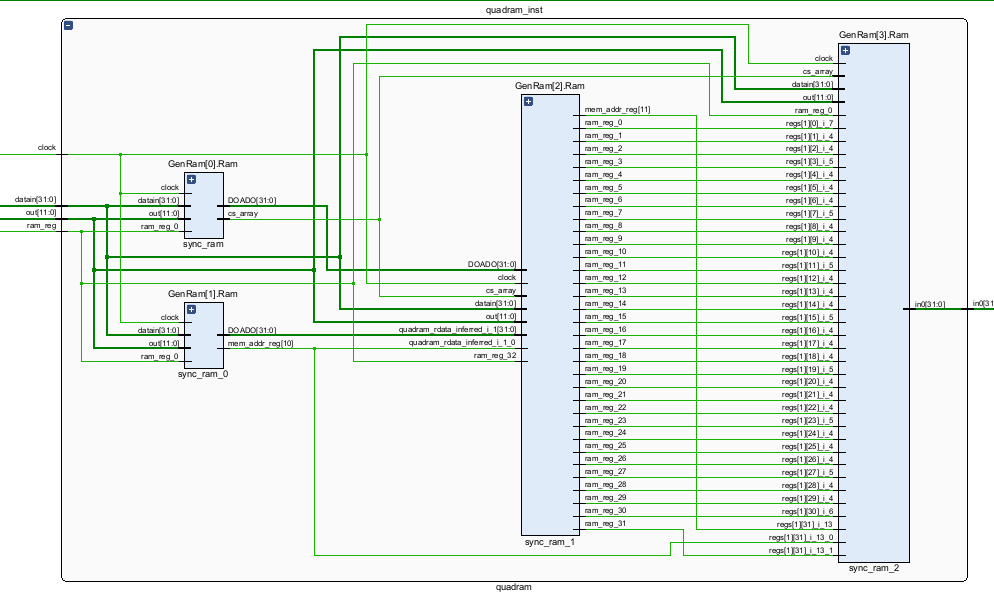
\includegraphics[width=\textwidth]{Images/6_Sche_Quadram.png}
        \caption{Vue du module QuadRAM}
        \label{fig:sche_quadram}
    \end{subfigure}
    \hfill
    \begin{subfigure}[b]{0.48\textwidth}
        \centering
        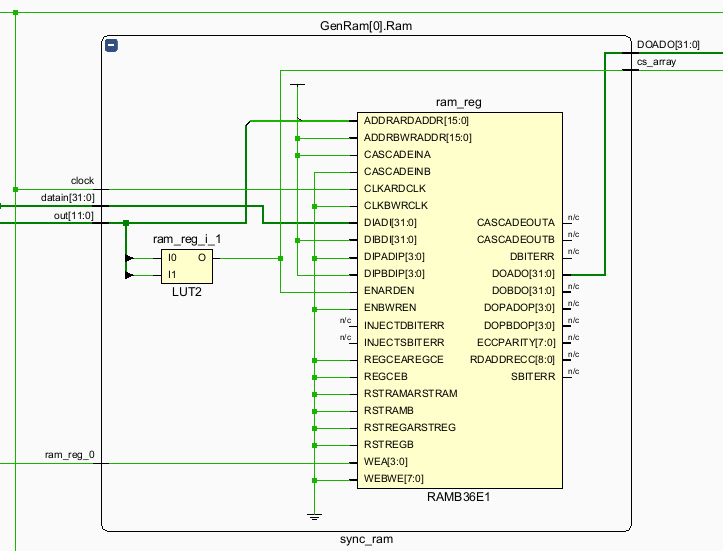
\includegraphics[width=\textwidth]{Images/6_Sche_gen0.png}
        \caption{Génération du design (\texttt{gen0})}
        \label{fig:sche_gen0}
    \end{subfigure}
    \caption{Vues schématiques de la synthèse sous Vivado}
\end{figure}

En zoomant sur la QuadRAM, nous pouvons observer les quatre blocs de mémoire RAM. La génération du design (\texttt{gen0}) met en évidence l'utilisation d'un bloc de mémoire interne au FPGA (RAMB36E1), optimisant ainsi l'utilisation des ressources logiques.

\begin{figure}[H]
    \centering
    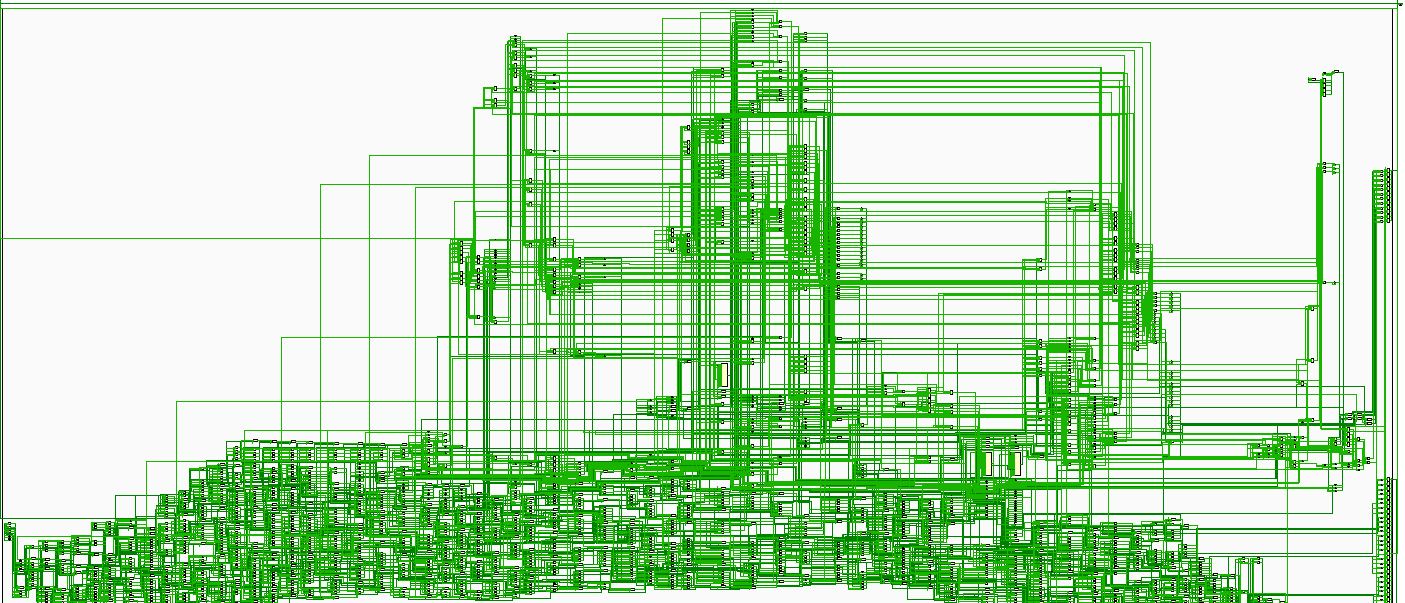
\includegraphics[width=0.99\textwidth]{Images/6_Sche_riscV.png}
    \caption{Vue du processeur RISC-V}
    \label{fig:sche_riscv}
\end{figure}

Le processeur RISC-V s'avère être le module le plus complexe à analyser en détail. Étant capable d'exécuter différentes opérations, ce schéma regroupe logiquement les différents sous-modules : l'unité arithmétique et logique (ALU), le décodeur d'instructions, le compteur ordinal (programme) et les registres internes.

\begin{figure}[H]
    \centering
    \includegraphics[width=\textwidth]{Images/6_Sche_ZoomProcessor.png.png}
    \caption{Zoom sur le processeur}
    \label{fig:zoom_processor}
\end{figure}

La figure ci-dessus présente un zoom sur une région spécifique du processeur, permettant d'observer la disposition des différents sous-modules internes.

\begin{figure}[htbp]
    \centering
    \begin{subfigure}[b]{0.48\textwidth}
        \centering
        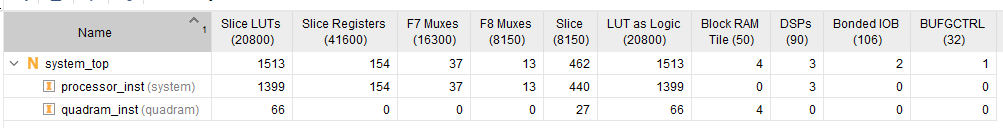
\includegraphics[width=\textwidth]{Images/6_UtilisationRessource.png}
        \caption{Rapport d'utilisation des ressources (1)}
        \label{fig:util_ressource}
    \end{subfigure}
    \hfill
    \begin{subfigure}[b]{0.48\textwidth}
        \centering
        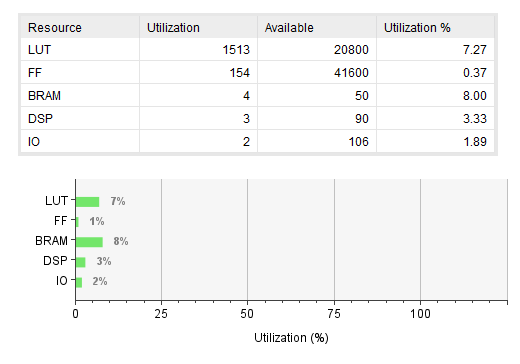
\includegraphics[width=\textwidth]{Images/6_utilisation_2.png}
        \caption{Rapport d'utilisation des ressources (2)}
        \label{fig:util_ressource_2}
    \end{subfigure}
    \caption{Rapports d'utilisation des ressources du design sous Vivado}
\end{figure}

Grâce au rapport d'utilisation des ressources, nous constatons que le design utilise seulement 7\,\% des LUTs et 1\,\% des FFs disponibles sur le FPGA. Cela témoigne de la légèreté de l'architecture, laissant une marge importante pour de futures extensions.

Au total, le design mobilise 1 513 LUTs, réparties entre 66 pour la QuadRAM et 1 399 pour le processeur. Cela confirme que ce dernier représente la majeure partie de la complexité logique du système, ce qui est cohérent avec la gestion des instructions et des accès mémoire.

\begin{figure}[htbp]
    \centering
    \begin{subfigure}[b]{0.48\textwidth}
        \centering
        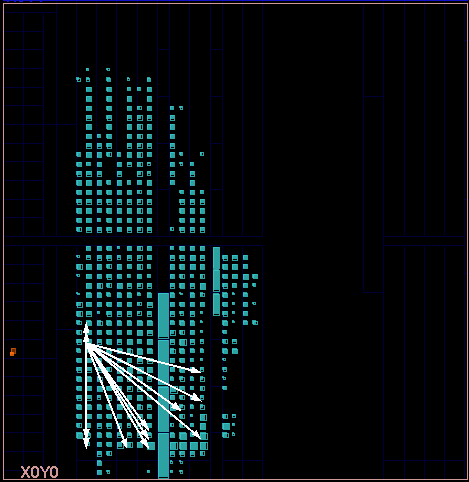
\includegraphics[width=\textwidth]{Images/6_Implentation.png}
        \caption{Vue de l'implémentation physique}
        \label{fig:implementation}
    \end{subfigure}
    \hfill
    \begin{subfigure}[b]{0.48\textwidth}
        \centering
        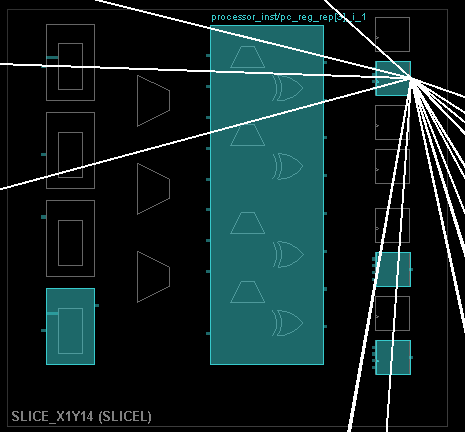
\includegraphics[width=\textwidth]{Images/6_zoom_implentation.png}
        \caption{Zoom sur le routage}
        \label{fig:zoom_implementation}
    \end{subfigure}
    \caption{Vues de l'implémentation et du placement-routage sur le FPGA}
\end{figure}

Enfin, l'implémentation physique du design sur le FPGA révèle la disposition spatiale des différents blocs. Le zoom sur le routage illustre les interconnexions réalisées par l'outil entre les blocs logiques. Nous pouvons notamment observer le signal \texttt{pc_reg_rep_0} (le registre de programme du processeur), issu directement d'une bascule D (\textit{D Flip-Flop}).